Following the completion of Run 3, the LHC will enter its third long shutdown (LS3). During LS3 the LHC and its major experiments will undergo massive upgrades in preparation for Run 4. For example, the LHC will upgrade numerous technologies such as the superconducting magnets, the radio frequency cavities, and the beam collimation systems~\cite{lhc_upgrade_run4}. The HL-LHC aims to deliver significantly more luminosity than it currently does in Run 3, expecting to sustain a luminosity of 5 to 7.5 times larger than the nominal LHC values. Along with the increased luminosity,
the energy of each proton beam is expected to have a \com{} of 7 TeV, producing proton-proton collisions with a \com{} of 14 TeV. 

Additionally, ATLAS will also be performing upgrades to their detector systems~\cite{atlas_detector_upgrade_run4}, data acquisition and trigger systems~\cite{atlas_detector_upgrade_run4}, as well as their computing and software infrastructure~\cite{CERN-LHCC-2022-005}. These upgrades, particularly those in software and computing, are critical to meet the demands of the HL-LHC era which is expected to bring higher event rates with over double the number of interactions per bunch crossing in comparison to Run 3, and over 10x more data collected than Run 1, 2 and 3 combined.
Figure~\ref{fig:atlas_cpu_usage} shows the expected CPU consumption required per year for ATLAS depending on two different R\&D scenarios. Aggressive R\&D assumes significant improvements in areas such as track reconstruction (e.g.\ a 20\% reduction in reconstruction time), a reduced amount full simulation events (reduced by 10\% to 30\%) and an increase in dedicated software and computing efforts, via new personnel or current personnel committing more time to development. In contrast, the conservative scenario assumes that current staff levels remain constant, no additional person-power and no loss of key experts.
Even with a sustained budget increase of 10\% for software and computing, neither scenario is expected to fully meet the CPU demands of the HL-LHC\@. However, if funding levels are increased by 20\% annually, the aggressive R\&D is projected to fulfill the required CPU capacity.

\begin{figure}[pht]
    \centering
    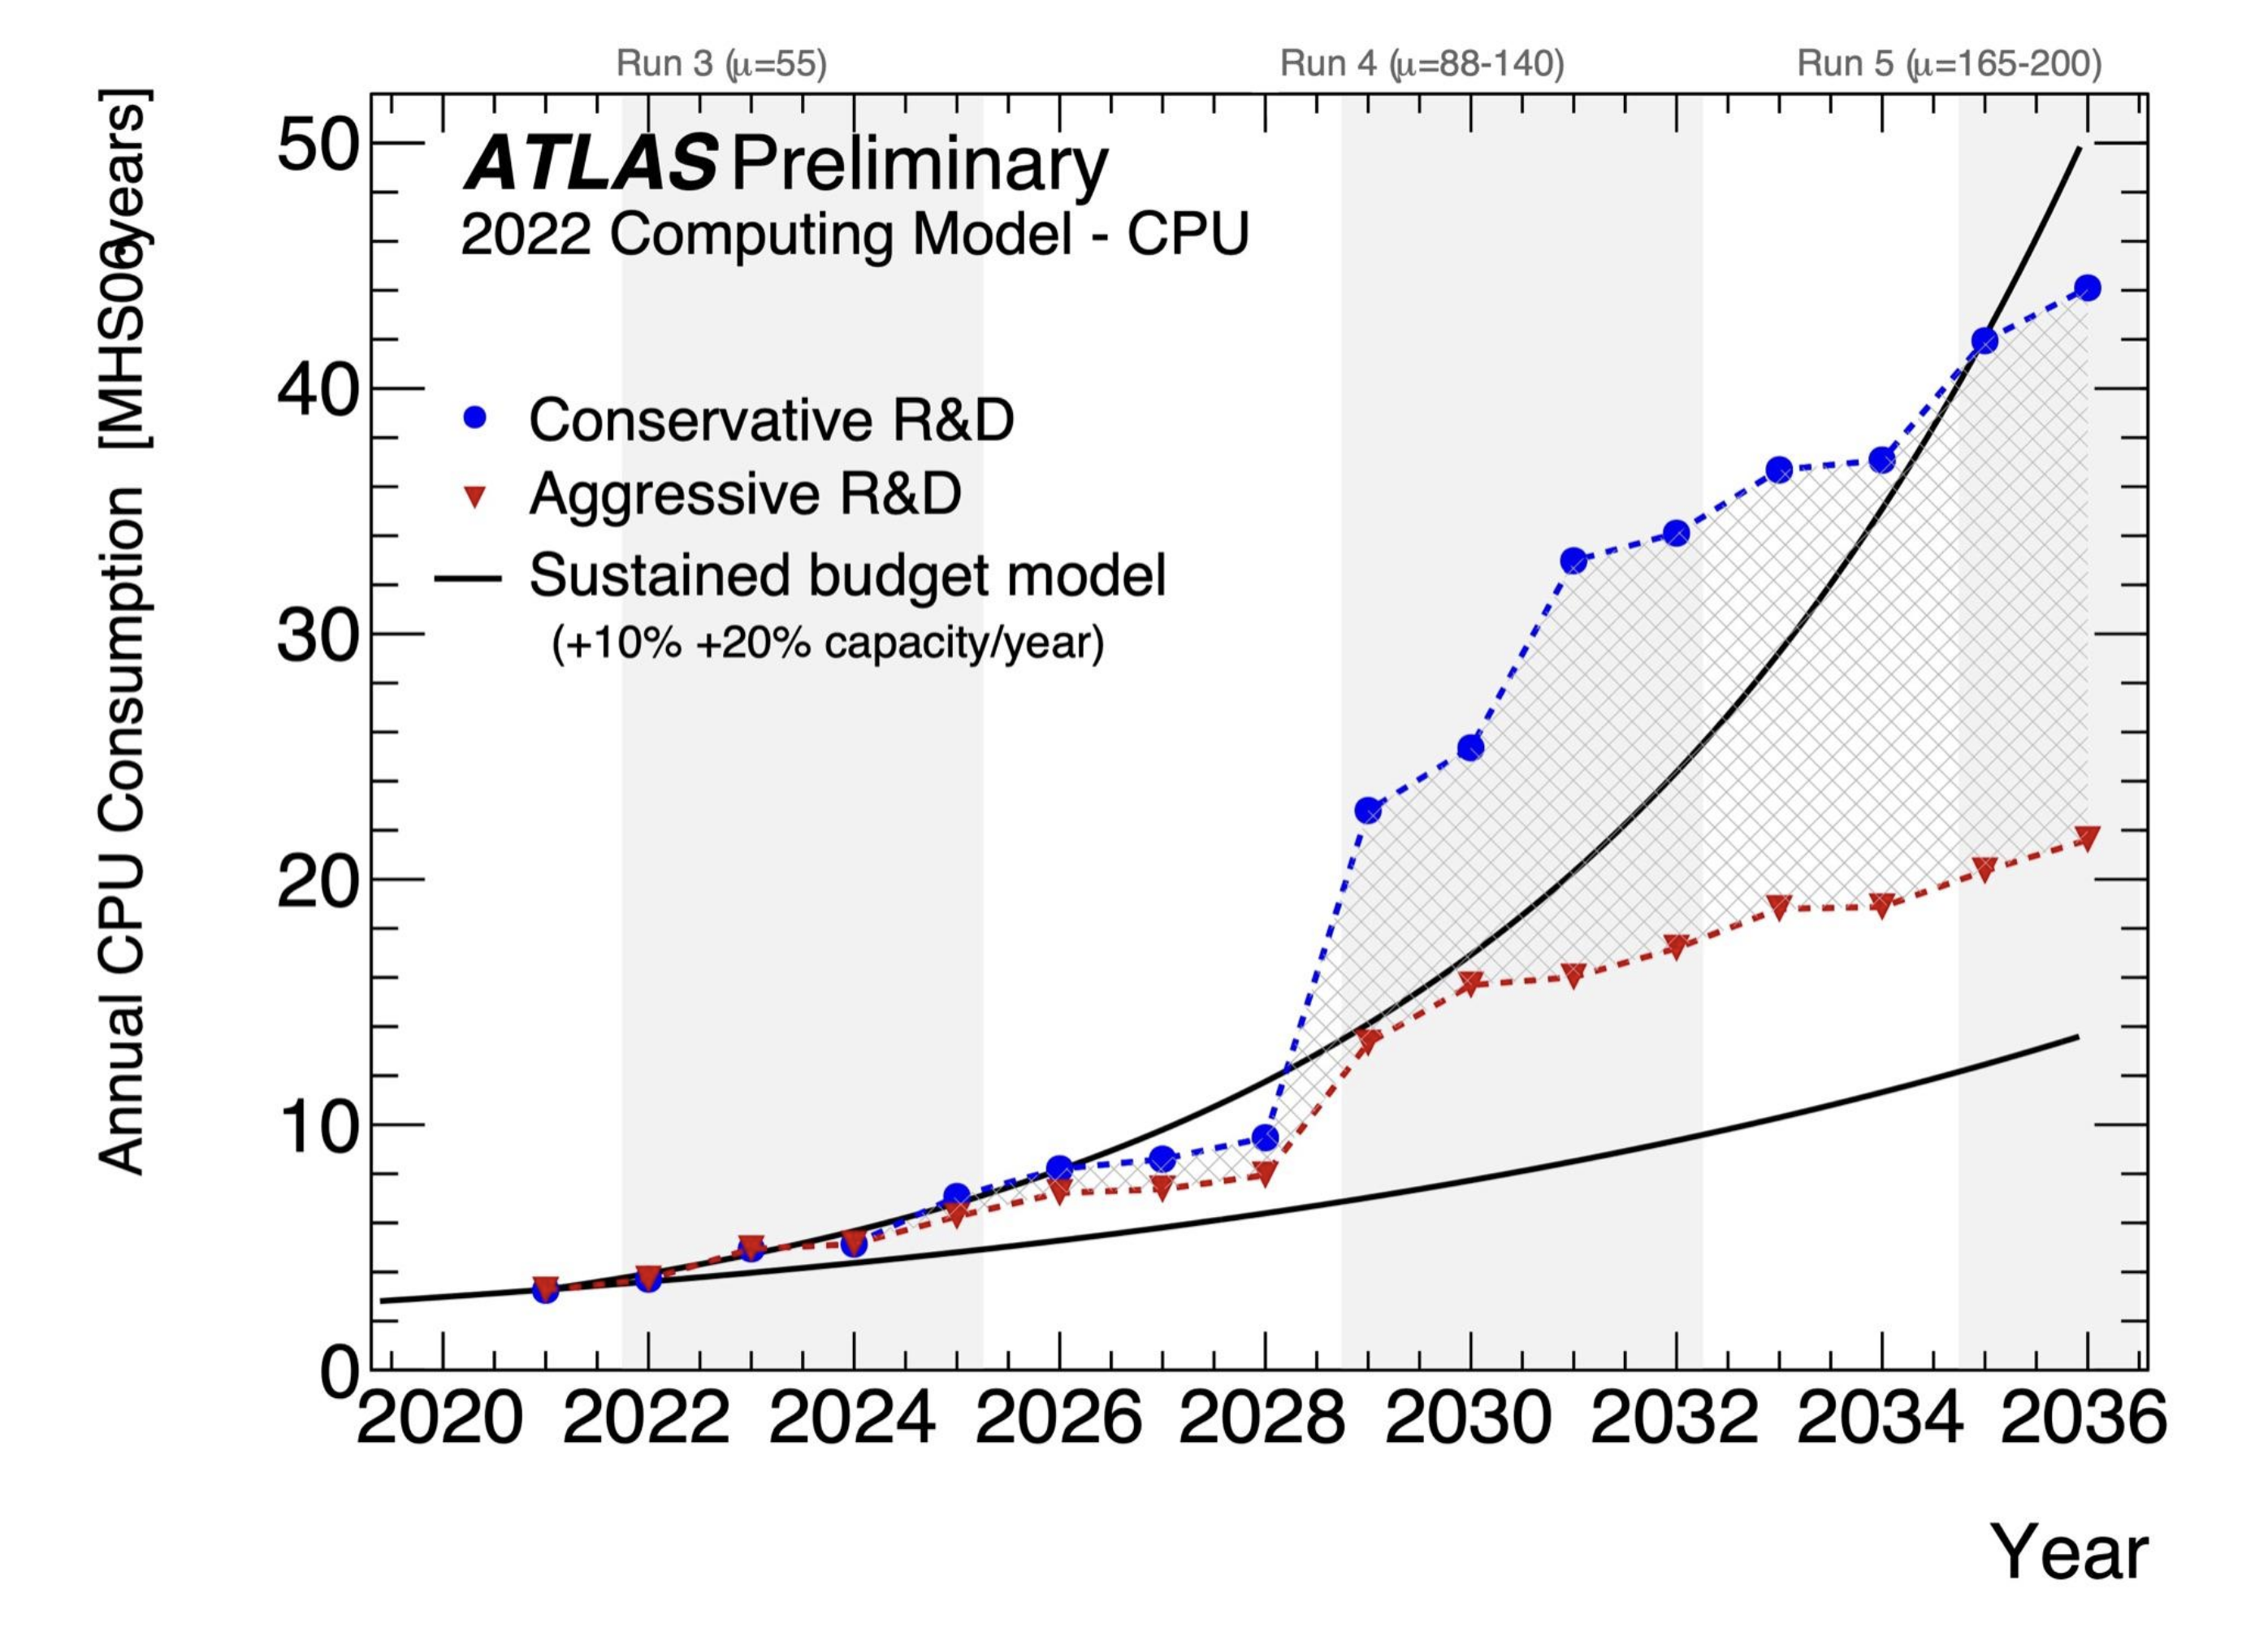
\includegraphics[width=0.9\textwidth]{figures/atlas/atlas_cpu_usage.png}
    \caption{The expected annual CPU usage for ATLAS during HL-LHC\@. The blue line shows the conservative R\&D scenario, which doesn't meet the anticipated demand for a 10\% or 20\% budget increase. The red line depicts the aggressive R\&D scenario and shows that with a 20\% budget increase yearly, the CPU demand can be fulfilled. Taken from~\cite{CERN-LHCC-2022-005}
    }\label{fig:atlas_cpu_usage}
\end{figure}

In this thesis, particular focus will be given to the software infrastructure developed for HL-LHC muon track reconstruction, which will be discussed in more detail in Chapter~\ref{ch:reco}.
